\documentclass{article}
\usepackage[left = 20mm, right = 20mm]{geometry}
\linespread{1.2}
\usepackage{xcolor,eso-pic,soul}
\usepackage{graphicx}
\usepackage{enumitem}
\usepackage{pifont}
\usepackage{hyperref}
\usepackage{mathtools}
\graphicspath{{./figures}}
\definecolor{bluunipv}{HTML}{1E489F}
\newcommand{\step}[1]{\underline{\textbf{\large{#1}}} }  
\setulcolor{bluunipv}
\setul{0.5ex}{0.3ex}
\title{\textcolor{white}{\textbf{Machine Learning per il Calcolo Scientifico}\\ \small\textbf{First laboratory exercises }}}
\date{}

% \AddToShipoutPictureBG{\color{bluunipv}%
% \AtPageUpperLeft{\rule[-20mm]{\paperwidth}{30cm}}%
% }

\begin{document}
    
    \definecolor{rossounipv}{HTML}{B2264A}
    \definecolor{bluunipv}{HTML}{1E489F}
    %\pagecolor{bluunipv}
    \AddToShipoutPicture*
    {%
      \AtPageUpperLeft
        {%
          \color{bluunipv}%
          \raisebox{-.1\paperheight}{\rule{\paperwidth}{.5\paperheight}}%

        }%
      %\color{white}%
     % \rule{\paperwidth}{.5\paperheight}%
    }
    \newgeometry{left = 20mm, right = 20mm, top = -6mm}
    \maketitle
    \begin{center}\step{General guide} \end{center}

    For each laboratory, an incomplete Python notebook will be provided with exercises (steps) that must be completed in the given order (some of the exercises will be needed in future laboratories). In step zero, all the Python packages that are needed in order to complete the notebook are listed. This PDF includes the text for the exercises and the expected outcomes for each step. While following the notebook is recommended, you are also welcome to attempt the exercises without using it.


    \begin{center}\step{Step Zero} \end{center}

    Here are the required Python (\url{https://www.python.org/}) packages for this laboratory:

    \begin{itemize}
      \item PyTorch (\url{https://pytorch.org/})
      \item Numpy (\url{https://numpy.org/})
      \item Matplotlib (\url{https://matplotlib.org/})
    \end{itemize}


    \begin{center}\step{First Step: Define $\Phi^\wedge$ using torch Tensors}\end{center}

    a. Using torch.tensor, define the weight and biases for the $\Phi^\wedge$ Neural Network (NN).
    
    b. Using the definition seen during the lecture construct the $\Phi^\wedge$ NN with ReLu activation that emulates $F_1$.
    \begin{center}
    $
      F_1 : x\mapsto 
      \begin{cases}
        2x &x\in (0, 1/2]\\
        2-2x &x \in (1/2, 1)\\
        0 &\text{elsewhere.}
      \end{cases}$
    \end{center}

    c. Plot the $\Phi^\wedge$ NN in [0,1].

    \begin{center}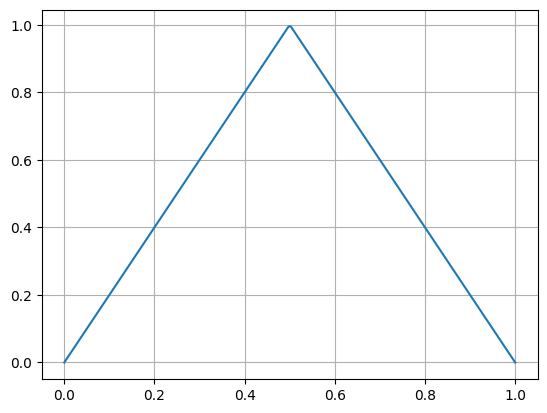
\includegraphics[scale = 0.5]{phi_wedge.png} \end{center}
    \newpage
    \restoregeometry
    \begin{center}\step{Second step: Define a general Feed-Forward Neural Network (FNN)}\end{center}
    
    a. Complete the Python class DeepNet that defines a general FNN in Pytorch. \textcolor{red}{(Will be used in other labs)} 
    
    b. Using the DeepNet class, create a FNN with 1 layer 3 neurons with ReLu as an activation function.

    \begin{center}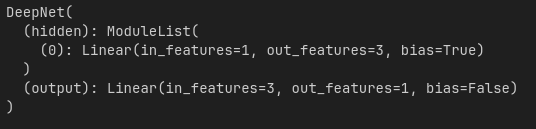
\includegraphics[scale = 0.5]{output_fnn.png}\end{center}
   
    c. Redefine the $\Phi^\wedge$ NN by loading the weights and biases defined in the first step point a (set\_weight set\_bias \newline \  \ set\_output\_weight) into the FNN. Then plot the output of the NN in [0,1].

    \begin{center}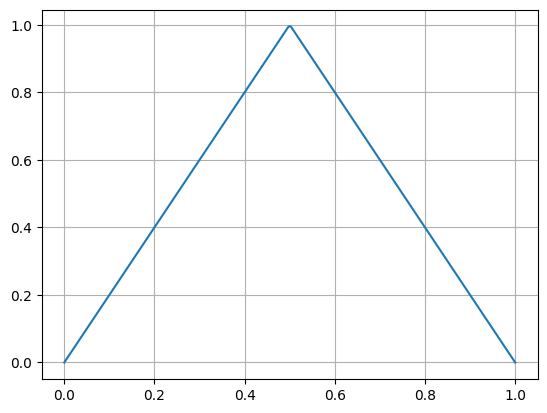
\includegraphics[scale = 0.5]{phi_wedge.png}\end{center}

  \begin{center}\step{Third step: Concatenation of two Networks}\end{center}
    
    a. Complete the Python function concatenate, which implements the non-sparse concatenation. 
    
    b. Concatenate 4 times the $\Phi^\wedge$ NN defined before (second step point c). 

    \begin{center}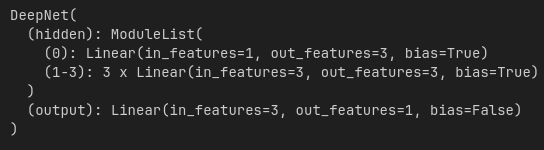
\includegraphics[scale = 0.5]{output_concatenate.png}\end{center}

    c. Plot the NN obtained in the previous point in [0,1].
    
    \begin{center}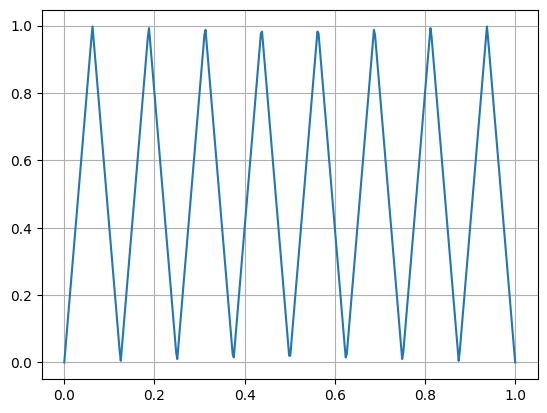
\includegraphics[scale = 0.5]{plot_concatenate.png}\end{center}

\begin{center}\step{Fourth step: Define the Yarotsky Network}\end{center}

    a. Complete the class YarotskyNet, then using this class define
    a Yarotsky NN with depth = 3.
  

    b. Plot the output of the Yarotsky Network over [0,1] and compare it to $x^2$.

    \begin{center}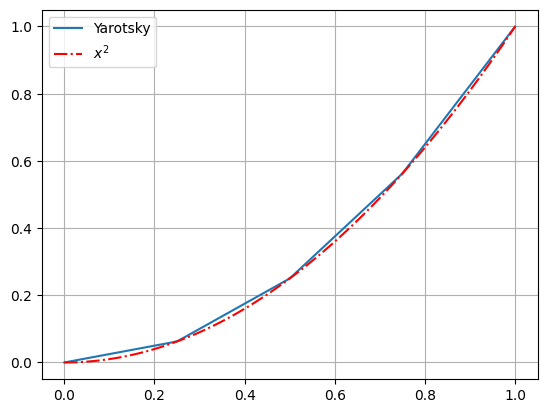
\includegraphics[scale = 0.5]{Yarotsky_comparison.png}\end{center}

    c. Evaluate the $L^2$ error of the Yarotsky NN with respect to $x^2$ ($\approx 1.13\times 10^{-2}$).

     
    d. Evalute the $L^2$ error of the Yarotsky Network with respect to $x^2$, as a function of the depth of the network.

    \begin{center}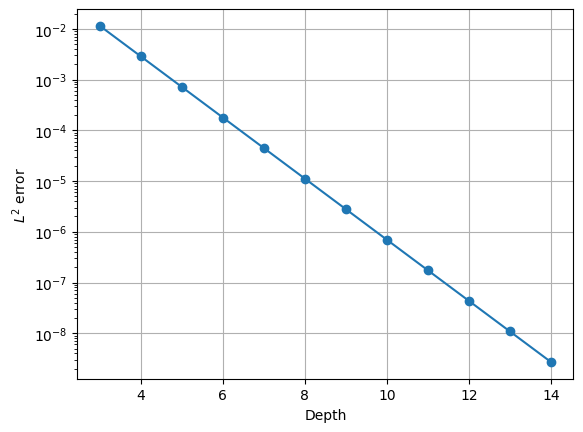
\includegraphics[scale = 0.5]{Yarotsky_convergence.png}\end{center}

  \end{document}
